\section{Example: The Dining Philosophers}

The Dining Philosophers problem is an example formulated by Edsger Dijkstra,
to illustrate some of the problems that can arise in concurrent programming.  
It is presented in terms of interactions between people; but it is an analogy
with concurrent threads or processes sharing resources. 

Five philosophers spend most of their lives thinking; but sometimes they need
to eat.  They share a common dining room, which has a circular table with five
chairs around it, a plate in front of each chair, and a big bowl of spaghetti
in the middle.  There are five forks, placed between the five plates at the
table.

When a philosopher gets hungry, they sit down.  They pick up the fork to their
left as soon as it's available (they might need to wait for their left-hand
neighbour to finish with the fork).  Then they pick up the fork to their right
as soon as it's available.  Once the philosopher has two forks, they serve
themself and spend some time eating.  They then put the forks down and do
some more thinking.

However, there is a problem with this protocol.  If all five philosophers get
hungry at about the same time and pick up their left fork, then they all
starve!  Of course, real philosophers---being smart people---would soon solve
the problem.  But if we think of this as an analogy for concurrent threads,
the program would not.  

We will build a simulation of the Dining Philosophers example.  We 
simulate each philosopher and each fork by a thread.  The first part of the
simulation is in Figure~\ref{fig:dining-phils-1}.

%%%%%%%%%%

\begin{figure}
\begin{scala}
/** Simulation of the Dining Philosophers example. */
object Phils{
  val N = 5 // Number of philosophers.

  // Simulate basic actions.
  def eat() = Thread.sleep(500)
  def think() = Thread.sleep(scala.util.Random.nextInt(900))
  def pause() = Thread.sleep(500)

  type Cmd = Boolean; val Pick = true; val Drop = false
 
  /** A single philosopher. */
  def phil(me: Int, left: !![Cmd], right: !![Cmd]) = thread(s"Phil $me"){
    repeat{
      think()
      println(s"$me sits"); pause()
      left!Pick; println(s"$me picks up left fork"); pause()
      right!Pick; println(s"$me picks up right fork"); pause()
      println(s"$me eats"); eat()
      left!Drop; pause(); right!Drop; pause()
      println(s"$me leaves")
    }
  } 

  /** A single fork. */
  def fork(me: Int, left: ??[Cmd], right: ??[Cmd]) = thread(s"Fork $me"){
    serve(
      left =?=> {x => assert(x == Pick); val y = left?(); assert(y == Drop)}
      |
      right =?=> {x => assert(x == Pick); val y = right?(); assert(y == Drop)}
    )
  } 
  ...
}
\end{scala}
\caption{The Dining Philosophers example (part 1).}
\label{fig:dining-phils-1}
\end{figure}

%%%%%%%%%%

We simulate the actions of eating and thinking, and a pause between other
actions, by having the thread sleep for a short period (the library method
|Thread.sleep(t)| suspends the current thread for |t|\,ms).

We can simulate the picking up and putting down of forks by the philosopher
thread sending a suitable value, |Pick| or |Drop|, respectively, to the fork
thread.  We denote the type of these values as~|Cmd|.  We choose to represent
the values as |Boolean|s.

The philosopher thread |phil| is parameterised by the philosopher's identity,
and out-ports on which it can send messages to its left- and right-hand forks.
The definition is then a straightforward translation of the earlier informal
description, sending |Pick| and~|Drop| messages to simulate the picking up and
dropping of the fork.  The code prints messages to the screen describing its
actions. 

The fork thread is parameterised by the fork's identity, and in-ports on which
it can receive messages from its left- and right-hand philosopher.  The fork
should initially be willing to receive a message on either of its in-ports,
which requires an alternation, in this case via a |serve| construct.  The
value it receives should be a |Pick|.  It then waits to receive a second
message on the same in-port, which should be a |Drop|.  The |assert|
statements check the correct messages are received.  Using assertions like
this is good practice.  If nothing else, it acts as good documentation.  But
such assertions can also help to catch mistakes.  I have found lots of
mistakes in my own code by including assertions like these.  If I had omitted
the assertions, it would probably have led to errors arising later in the
program, but it would have been much harder to identify the cause of the
problem.

We connect the philosophers and forks together as depicted in the top half of
Figure~\ref{fig:dining-philosophers-2}, with the corresponding code in the
bottom half of the figure.  We use two arrays of channels, indexed by the
identities of the philosophers: channel |philToLeftFork(i)| is from |phil(i)|
to |fork(i)|; and channel |philToRightFork(i)| is from |phil(i)| to
|fork(|$(\sm i-1) \bmod \sm N$|)|.  It is easy to get confused about the
indexing of arrays of channels in cases like this: I recommend drawing a
picture and writing a clear comment.  

%%%%%%%%%%

\begin{figure}
\begin{center}
\def\r{4.07}
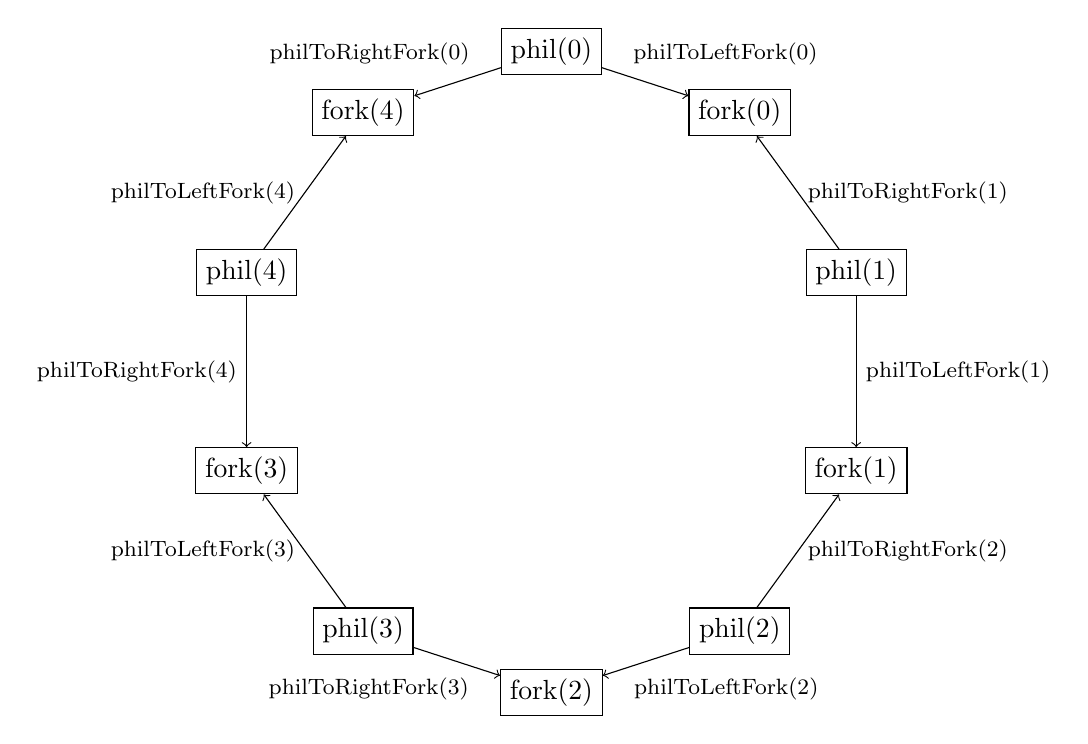
\begin{tikzpicture}
\foreach \i in {0,...,4} 
  \draw (90-72*\i: \r) node[draw] (phil\i) {\scalashape phil(\i)}; 
\foreach \i in {0,...,4} 
  \draw (54-72*\i: \r) node[draw] (fork\i) {\scalashape fork(\i)}; 
%
\draw[->] (phil0) -- node[above right, near start] 
  {\scalashape\footnotesize philToLeftFork(0)} (fork0);
\draw[->] (phil1) -- node[right] 
  {\scalashape\footnotesize philToLeftFork(1)} (fork1);
\draw[->] (phil2) -- node[below right, near end] 
  {\scalashape\footnotesize philToLeftFork(2)} (fork2);
\draw[->] (phil3) -- node[left] 
  {\scalashape\footnotesize philToLeftFork(3)\ } (fork3);
\draw[->] (phil4) -- node[left] 
  {\scalashape\footnotesize philToLeftFork(4)\ } (fork4);
%
\draw[->] (phil0) -- node[above left, near start]
  {\scalashape\footnotesize philToRightFork(0)} (fork4);
\draw[->] (phil1) -- node[right]
  {\scalashape\footnotesize philToRightFork(1)} (fork0);
\draw[->] (phil2) -- node[right]
  {\scalashape\footnotesize philToRightFork(2)} (fork1);
\draw[->] (phil3) -- node[below left, near end]
  {\scalashape\footnotesize philToRightFork(3)} (fork2);
\draw[->] (phil4) -- node[left]
  {\scalashape\footnotesize philToRightFork(4)} (fork3);
\end{tikzpicture}
\end{center}

%%%%%

\begin{scala}
  /** The complete system. */ 
  def system = {
    val philToLeftFork, philToRightFork = Array.fill(N)(new SyncChan[Cmd])
    // £philToLeftFork(i)£ is from £phil(i)£ to £fork(i)£;
    // £philToRightFork(i)£ is from £phil(i)£ to £fork($(\sm i-1) \bmod \sm N$)£.
    val allPhils = || ( 
      for (i <- 0 until N) yield phil(i, philToLeftFork(i), philToRightFork(i))
    )
    val allForks = || ( 
      for (i <- 0 until N) yield
        fork(i, philToRightFork((i+1)%N), philToLeftFork(i))
    )
    allPhils || allForks
  }

  /** Run the system. */
  def main(args : Array[String]) = run(system)
\end{scala}
\caption{The Dining Philosophers example (part 2).}
\label{fig:dining-philosophers-2}
\end{figure}

%%%%%%%%%%%

It is important that we use \emph{synchronous} channels: we need each
philosopher and fork to synchronise on relevant actions. 

When we run the system, sometimes it deadlocks almost immediately.  A typical
deadlocking trace is:
%
\begin{scala}
1 sits,  0 sits,  4 sits,  2 sits,  1 picks up left fork, 3 sits,  0 picks up left fork,  
4 picks up left fork, 2 picks up left fork,  3 picks up left fork
\end{scala}
%
Each philosopher sits down and picks up their left fork (in some order).  At
this point, each philosopher is trying to pick up its right fork, i.e.~to send
a |Pick| message on its |right| channel; however, the corresponding fork is
not willing to receive that message.  This means that the system is
deadlocked.

Recall that typing \texttt{Ctrl}+$\backslash$ gives a thread dump.  This will
give the line number in the code where each thread is stuck, so can help to
understand the deadlock.   

However, sometimes when we run the system, it runs for a very long time
without deadlocking.  In fact, I chose the delays in the simulations of the
basic actions so that the system deadlocks about half the time.  Different
choices for these delays would have caused the system to deadlock on nearly
every run, or hardly ever.  In some ways, the latter situation is worse: it is
likely that the potential deadlock would not be found by testing, but that it
occurs only when the system is deployed.

%%%%%%%%%%

\subsection{Logging}

In the above simulation, we used |println| statements so that we could
understand what happened.  However, this style is often not convenient.
Normally, a better way is to use logging.

The SCL class |Log| provides log objects.
%
A new log storing events of type~|A|, suitable for |p| threads,
can be defined by
\begin{scala}
  val log = new Log[A](p)
\end{scala}
%
This provides operations
%
\begin{itemize}
\item |def add(me: Int, x: A)|, which adds |x| to the log,
performed by thread~|me|;

\item |def get: Array[A]|, which gets the contents of the log;

\item |def toFile(fname: String = "/tmp/logFile")|, which writes the contents
  of the log to the file~|fname| (with a default of \texttt{/tmp/logFile}).
\end{itemize}

The code below shows how we can use logging in the dining philosophers
example.
%
\begin{scala}
  val log = new Log[String](N)
 
  def phil(me: Int, left: !![Cmd], right: !![Cmd]) = thread(s"Phil $me"){
    repeat{
      think()
      log.add(me, s"$me sits"); pause()
      left!Pick; log.add(me, s"$me picks up left fork"); pause()
      right!Pick; log.add(me, s"$me picks up right fork"); pause()
      log.add(me, s"$me eats"); eat()
      left!Drop; pause(); right!Drop; pause()
      log.add(me, s"$me leaves")
      if(me == 0) print(".")
    }
  }
\end{scala}
%
(I have arranged for philosopher~|0| to print a dot on each iteration, so we
can tell whether the system is making progress.)

In many scenarios, when the system terminates, we can either write the log to
a file, or analyse the log using some code.  However, this won't work when the
system deadlocks.  Instead, we need to insert a hook that will arrange for the
log to write itself to a file when the user interrupts the program.  This can
be done with the |writeToFileOnShutdown| method:
%
\begin{scala}
  def main(args: Array[String]) = {
    log.writeToFileOnShutdown("philsLog.txt"); run(system)
  }
\end{scala}

Logging is a general technique that can help with debugging.  However, there
is a wrinkle concerning its usage.
%
Internally, each thread uses its own thread-local log, to avoid race
conditions, and for efficiency.  Each logged value is stored in the relevant
thread-local logs, together with a timestamp (more precisely, the time elapsed
since the |Log| object was created, to avoid problems with timestamp
wrap-around).
%
The |get| operation merges the thread-local logs according to
timestamps.

Using timestamps in this way assumes that the clocks are loosely synchronised
across cores, and that the granularity of the clocks is sufficiently fine, so
that if one |add| event logically happens before another (i.e.~according to
the~$\prec$ relation), the former receives a strictly smaller timestamp.

The above assumption seems to be sound in Linux, but not in Windows.  If you
must use Windows, the class |SharedLog| provides the same interface.  However,
it will give worse performance.  Further, it might affect the likelihood of
detecting bugs: I have experienced bugs that would appear when no logging was
performed, or when the timestamp-based log was used; but logging with
something equivalent to |SharedLog| affected the speed of threads sufficiently
that the bug would no longer appear in a reasonable time!


%%%%%%%%%%%%%%%%%%%%%%%%%%%%%%%%%%%%%%%%%%%%%%%%%%%%%%%

\subsection{Avoiding deadlocks}
\label{sec:avoid-deadlocks}

\def\waitingFor{\vdash}

The deadlock in the dining philosophers example corresponds to a cycle of
waiting.  Each philosopher is trying to pick up their right-hand fork, and is
waiting for that fork.  Each fork is waiting for their right-hand philosopher
to put it down.  Let's write $t_1 \waitingFor t_2$ to signify that thread
$t_1$ is blocked, waiting for thread~$t_2$.  Then we have the following cycle
of waiting:
\[\mstyle
\sm{phil}(0) \waitingFor \sm{fork}(4) \waitingFor \sm{phil}(4) \waitingFor
  \sm{fork}(3) \waitingFor \ldots \waitingFor \sm{fork}(0) \waitingFor
  \sm{phil}(0).
\]
This corresponds to an anti-clockwise cycle in
Figure~\ref{fig:dining-philosophers-2}.

In fact, deadlocks correspond to cycles of waiting more generally.  Consider a
system based on message passing, and suppose that for every channel~$c$, there
is some thread that sometimes sends on~$c$, and some thread that sometimes
receives on~$c$ (or else the system is badly configured).  Consider a
deadlocked state, and suppose no thread has terminated or is performing an
infinite amount of internal computation.  Then necessarily every thread is
trying to send or receive on a channel.  Pick a thread $t_1$.  It is trying to
send or receive on some channel~$c_1$, so necessarily there is some
thread~$t_2$ that sometimes receives or sends (respectively) on~$c_1$; hence
$t_1$ is waiting for~$t_2$, i.e.~$t_1 \waitingFor t_2$.  By the same argument,
there is some thread $t_3$ such that $t_2 \waitingFor t_3$.  Continuing in
this way, we can construct an infinite sequence of threads such that each is
waiting on the next.  However, there are necessarily finitely many threads, so
this infinite sequence must contain the same thread twice, which constitutes a
waiting cycle.

If the system uses an alt, then a thread may be waiting for either of two or
more threads.  For example, in the dining philosophers example, a fork in its
initial state is waiting for either its left- or right-hand philosopher
(although there is no deadlocked system state corresponding to this state for
the fork).  In such cases, a deadlocked state may contain multiple waiting
cycles, and breaking any one of them would remove the deadlock.  A similar
fact is true when a channel is shared by several receivers, so a sender might
be waiting for any one of those receivers; and similarly when a channel is
shared by several senders.

There are a couple of ways of adapting the dining philosophers example so as
to remove the possibility of deadlock.  Each involves removing the possibility
of a waiting cycle.  Exercise~\ref{ex:diningPhils} asks you to implement
these. 

Note that whenever a philosopher is holding a fork but trying to drop it, that
action is never blocked.  Thus a philosopher that is waiting must be trying to
pick up a fork, but that fork is held by another philosopher.  That fork,
then, is waiting for the latter philosopher to drop it.  And the latter
philosopher must be waiting to pick up the next fork.  Continuing in this way,
we see that any waiting cycle must involve \emph{all} the philosophers and
forks. 

One way to avoid deadlocks is to introduce a ``butler'' thread that ensures
that there are never more than four philosophers seated.  We argue by
contradiction that there is then no deadlocked state.  Suppose otherwise.  Not
all philosophers can be seated, by design.  Without loss of generality,
suppose philosopher~$0$ is not currently seated.  Then necessarily that
philosopher cannot be holding fork~$0$ or fork~$4$.  But this then removes the
possibility of a waiting cycle, because neither of those forks is waiting for
philosopher~$0$.  This contradicts the observation in the previous paragraph
that any waiting cycle most involve all the threads.

In the earlier version of the dining philosophers example, all philosophers
picked up their left fork before their right fork.  Another way to avoid the
deadlock is for some (but not all) of the philosophers to pick up their right
fork first.  If that is the case, there must be an adjacent pair of
philosophers neither of whom picks up their shared fork first.  Without loss
of generality, suppose philosopher~$0$ picks up fork~$4$ before fork~$0$, and
philosopher~$1$ picks up fork~$1$ before fork~$0$.  This then removes the
possibility of a waiting cycle.  If either philosopher~$0$ or philosopher~$1$
holds fork~$0$ then they necessarily hold their other fork, and so can drop a
fork.  Otherwise, neither philosopher holds fork~$0$, so that fork cannot be
part of a waiting cycle.

Another way to avoid deadlocks is to detect that a potential deadlock has been
reached, and to react to remove that possibility, by backtracking.  For
example, if a philosopher holds one fork, but is unable to pick up their
second fork, they could drop their first fork, and try again later (this is
probably how real philosophers would act).

Within SCL, this could be achieved using a timeout.  Each channel has an
operation
%
\begin{scala}
  def sendWithin(millis: Long)(x: A): Boolean 
\end{scala}
%
This tries to send~|x| for up to |millis| milliseconds; but if no receiver is
ready within that time (or no space is available, in the case of a buffered
channel), it times out.  The operation returns a |Boolean| to indicate whether
the send was successful.  Likewise there is an operation
%
\begin{scala}
  def receiveWithin(millis: Long): Option[A] =
\end{scala}
%
that tries to receive a value for up-to |millis| milliseconds.  If it
successfully receives a value~|x|, the operation returns~|Some(x)|; otherwise
it returns~|None| to indicate a timeout.  There are also operations
|sendWithinNanos| and |receiveWithinNanos| where the time is given in
nanoseconds.
